\chapter{Evaluation}
\section{Experiments and Measurements}
\subsection{Experiment A: Orchestral Concert to Analyze Musical Absorption using Nidra to Collect Breathing Data}
The experiment was conducted in collaboration with master student Joachim Dalgard at the University of Oslo at the faculty of \textit{RITMO: Centre for Interdisciplinary Studies in Rhythm, Time and Motion}. 

The goal of the experiment was to analyze musical absorption, which is a state an individuals ability and willingness allows music to draw them into an emotional experience and becomes unaware of time and space. In order to analyze the effect of musical absorption on individuals, we gathered 20 participants who were experienced listeners with musical education. The participants attended an orchestral concert by Richard Strauss' Alpine Symphony---a symphonic poem that portrays the experience of eleven hours spent climbing an Alpine mountain---that lasted around 50 minutes at Oslo Concert Hall on third of April and fourth of April 2019.  

The participants were divided into two groups to attend the concert on the two dates. Each participant was equipped with a wireless electromyographic sensor from DELSYS in order to measure heart rate, and a Flow sensor kit to measure respiration during the concert. RITMO had multiple Flow sensors for disposal; however, they had no suitable mobile application that could record with these sensors. Also, with their equipment they experienced that Flow sensor kits tended to disconnect every 10-15 minutes, resulting in fragmented recordings for a single session. Therefore, they reached out to \textit{Insitute for Informatics} in hopes of a solution. Our application was a suiting match for both parties, hence a collaboration was formed. We arranged for six Android devices and reached out to the participants to bring their Android devices if they had one. There were ten participants in each group and six assessed devices. As a precaution, we decided to give out the devices to the participants who scored highest on a test performed on beforehand.

The motivation for this experiment in regards to Nidra was to test the application in a real-life and crowded environment. During the concert, there were approximately 800 attendees on the first day and approximately 1500 attendees on the second day. We can assume that most of the attendees had a mobile device, and a few shares of them had BlueTooth activated on the device. Based on these estimates, we were able to replicate an environment (on a larger scale) where other devices might interfere with the signals between the collecting sensor and the application. Also, we were able to install the application on multiple mobile devices with different Android OS versions and put the application in the hands of the participants. 

\subsubsection{Preperations}

\begin{table}
\begin{center}
\scalebox{0.59}{
\begin{tabular}{ |c|c|c|c| } 
\hline
\textbf{Model} & \textbf{Samsung Galaxy S9} & \textbf{OnePlus 3T} & \textbf{Google Pixel XL} \\
\hline
Operating System & Android 8.0 & - & Android 9.0 \& Android 7.1.2  \\
Chipset & Exynos 9810  & Qualcomm MSM8996 Snapdragon 821 & Qualcomm MSM8996 Snapdragon 821  \\
CPU & Octa-core & Quad-core & Quad-core \\
GPU & Mali-G72 MP18 & Adreno 530 & Adreno 530  \\
RAM & 4 GB & 6 GB & 4 GB \\
Battery & Li-Ion 3000 mAh & Li-Ion 3400 mAh & Li-Ion 3450 mAh  \\
Bluetooth & 5.0, A2DP, LE, aptX & 4.2, A2DP, aptX HD, LE & 4.2, A2DP, LE, aptX \\

\hline
\end{tabular}}
\caption{Device models used during the concert}
\end{center}
\end{table}

In order to partake in the experiments, we had to ensure that the participants had the sensor placed correctly on their body and the mobile devices were configured correctly. Also, stress testing the application to prevent any unforeseen events or bugs during recording. 

\begin{description}
    \item[Device Configuration] The device models in our disposal had to be configured with the applications to enable recording on Nidra. First, the data stream dispatching module was installed on the devices. Second, the sensor wrapper for the Flow sensor kit was configured with the respective sensor (in order to reduce the time on to set up the mobile device and the sensor on the participant). Lastly, the Nidra application was initiated with appropriately user information, in order to distinguish each participant with the sensor and device model. In Figure 6.1, the device models are listed with their specifications and the OS ... [Skriv mer]
    \item[Body Placement] The respiration value is based on the participant body circumference, and changes are associated with breathing. The participant was instructed to place the sensor around their thorax (just below the armpits), in order to measure the expansion and contraction of the rib cage.

\end{description}

\subsubsection{Results}

We gathered all of the data from the devices by using the sharing functionality in the application and sent it to our application. There were thirteen mobile devices combined for both dates---the other device was from one of the participants---however, the application crashed on one of the mobile devices during the recording. Therefore, we have access to twelve recordings from the concerts. 

\begin{figure}
\parbox{7cm}{
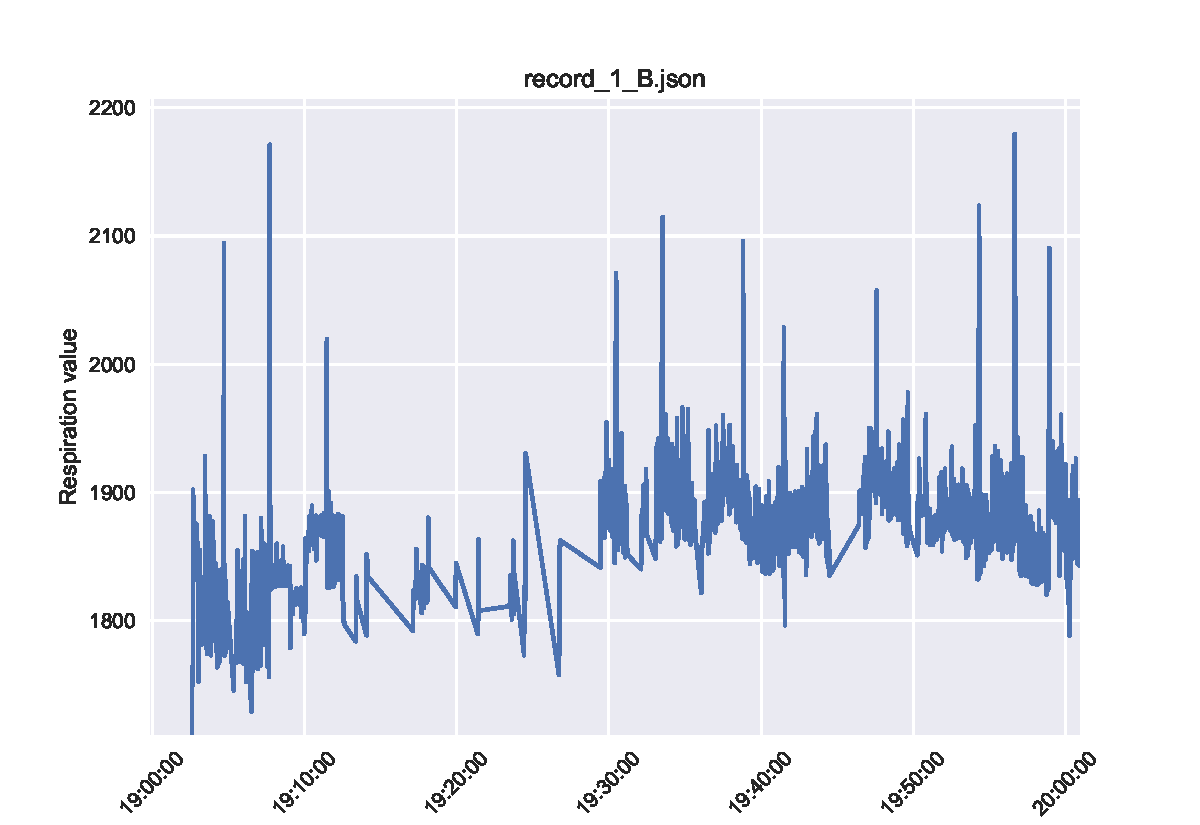
\includegraphics[width=8cm]{images/Record_1_B.pdf}
\caption{Concert Day 1---Mobile Device B}
\label{fig:day_1}}
\qquad
\begin{minipage}{6cm}
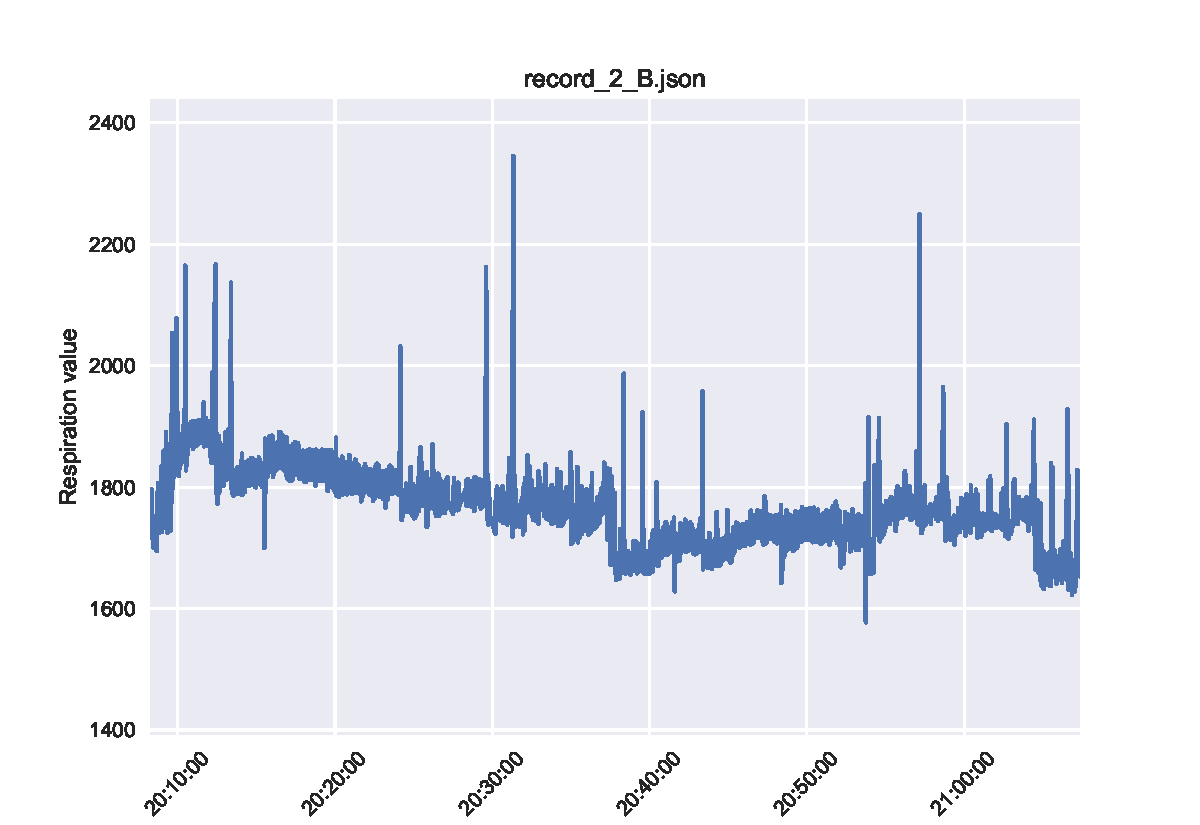
\includegraphics[width=7cm]{images/Record_2_B.pdf}
\caption{Concert Day 2---Mobile Device B}
\label{fig:day_2}
\end{minipage}
\end{figure}

Figure \ref{fig:day_1} and Figure \ref{fig:day_2} present two of these twelve recordings (rest can is found in Appendix B) that are of most interest to us in a time-series graph. The Y-axis represents the respiration (breathing) value, and the X-axis the time of respiration value acquisition---\textit{day one} of the concert started at the time of 19:00 and ended at 20:00, while \textit{day two} started at the time of 20:10 and ended 21:00. The graphs are plotted with Python and the library MatPlotLib in order to analyze and evaluate the graphs; however, an identical graph is also presented in the application.

From the figures, we can see that the respiration value is stable with some fluctuations and disconnections. Disconnections are defined as when the line is sloping or benching in an extended period (e.g., 20 seconds or more), while fluctuations are samples that spikes in the graph. Also, the respiration value can vary through the recording based on body position (e.g., sitting relax or tense in a chair). From the thesis "..." by Løberg, we can group the signals strengths based on four types of breathing patterns: (1) normal breathing---normal exhaling and inhaling (12-18 breaths per minute); (2) no breathing---close to flat rates over a long period; (3) shallow breathing---rapid inhaling and exhaling; and (4) deep breathing---prolonged inhaling or exhaling.

Figure 6.1 has many disconnects (further analyzed later) with unstable breathing---unstable breathing can occur due to body or sensor movement. There are multiple occurrences of deep breathing throughout the recording, with some shallow breathing at the start and the end of the recording. 

Figure 6.2 has fewer disconnects compared to Figure 6.2, and with much concise breathing patterns. The whole recording has a resemblance to deep breathing with few shallow breathings, but mostly a stable breathing pattern.

Conclusively, based on analyzing the two recordings done on the same devices, no nuances for no breathing was captured. However, instances of normal breathing, with few occurrences of shallow and deep breathing can be seen. We will further analyze all of the recordings in the next Subsection. 

\subsubsection{Analysis \& Discussion}
We will discuss all twelve records by analyzing the respiration values. It is of interest to find occurrences of disconnects---when the samples are stagnant in more extended period---and the time the sensor is disconnected during the recording.

\begin{table}[!h]
\begin{center}
\scalebox{0.7}{
\begin{tabular}{ |c|c|c|c||c|c| } 
\hline
\textbf{Model} & \textbf{Samples Count} & \textbf{Loss Count} & \textbf{Loss Percentage} & \textbf{Disconnection Count} & \textbf{Disconnection Time} \\
\hline
A & 5145 & 0 & 0 \% & 0  & 00:00  \\
\hline
B & 3363 & 1782 & 34 \% & 13 & 19m:14s  \\
\hline
C & 4189 & 956 & 19 \% & 7 & 8m:20s  \\
\hline
D & 3501 & 1644 & 32 \% & 5 & 18m:30s  \\
\hline
E & 5144 & 1 & 0.02 \% & 0 & 00:00  \\
\hline
F & 5145 & 0  & 0 \% & 0 & 00:00  \\
\hline
\end{tabular}}
\caption{Day 1---Duration: 1 hour \& Roof Samples: 5145}
\end{center}
\end{table}


\begin{table}[!h]
\begin{center}
\scalebox{0.7}{
\begin{tabular}{ |c|c|c|c||c|c| } 
\hline
\textbf{Model} & \textbf{Samples Count} & \textbf{Loss Count} & \textbf{Loss Percentage} & \textbf{Disconnection Count} & \textbf{Disconnection Time} \\
\hline
A & 4286 & 2 & 0.05 \% & 0  & 00:00  \\
\hline
B & 4161 & 127 & 3 \% & 4 & 1m:25s  \\
\hline
C & 4286 & 2 & 0.05 \% & 0 & 00:00  \\
\hline
D & 2576 & 1712 & 40 \% & 7 & 24m:35s  \\
\hline
E & 4285 & 3 & 0.06 \% & 0 & 00:00  \\
\hline
F & 4288 & 0  & 0 \% & 0 & 00:00  \\
\hline
\end{tabular}}
\caption{Day 2---Duration: 50 mins. \& Roof Samples: 4288}
\end{center}
\end{table}

The recordings for the six devices for the two dates are represented in Table 6.2 and Table 6.3. Each table exhibits data that is extracted from each recording from the mobile device and can be characterized as: 

\begin{description}
    \item[Roof Sample] The expected number of samples that can be acquired in the period of the recording (based on the frequency of sample output by Flow Sensor).
    \item[Sample Count] The number of samples that were gathered in the duration of the recording. 
    \item[Loss Count] The number of missing samples based on \verb|Roof Samples|. This can be calculated as: 
\begin{equation} \label{losscount}
Loss\ Count = Roof\ Samples - Samples
\end{equation}
    \item[Loss Percentage] The percentage of missing samples based on the expected samples. This can be calculated as:
\begin{equation} \label{losscount}
Loss\ Percentage = (1 - \frac{Samples}{Roof\ Samples}) * 100
\end{equation}
    \item[Disconnection Count] Is the number of disconnections that occurred within the duration of the recording.
    \item[Disconnection Time] Is the accumulated time of disconnection. 
\end{description}

The device models A, E, and F are noticeably accurate (with some noises which presumably occurred during parsing), there are no apparent disconnects occurred during the recording for these models both of the days. In contrast, device model B, C, D shows an outburst of disconnections during recording. Especially, model D has high loss percentage both of the days, which is reflected in the disconnection time. Also, model B had a high loss percentage on the first day; however, significantly less loss percentage the second day. 



\subsubsection{Conclusion}
To summarize this experiment, we were able to test the application in a real-life and crowded environment. The application managed to record samples that lasted up to 1 hour with the Flow senor and various device models with different Android OS versions. However, one of the application crashed, and we were unable to find the source of the problem. Based on samples from the recording, it is identified that the Flow sensor has a tendency of disconnecting, but the application managed to provide a continuous data stream by reconnecting with the sensor during recording. In the end, the records were successfully shared between the devices, in order to accomplish this analysis.  

To conclude, the goal of the experiment was to analyze musical absorption during a concert, but that is out of the scope for this thesis. However, we provided an application that collected the data during the concert. Thus, the collected data can then be used to conclude a correlation between breathing and musical absorption. Also, inconsistency in the sampling of the recordings makes it difficult to determine the source of the problem. We could argue that the analysis of the aggregated data in the tables might indicate that the sensor or the mobile is a malfunctioned, however, due to insufficient data this conclusion cannot be drawn. Although, the application managed to collect data with the use of the Flow sensor kit, in an environment filled with other mobile devices that could have interfered with the signals, as well as reconnecting to the sensors during the recording.

\subsection{Experiment B: 8-hours recording}
\subsection{Experiment C: User-Experience}

\subsection{Experiment D: Creating a Simple Module}



\section{Main Findings}
